\chapter{Environments}\label{environments}

The environment is the data structure that powers scoping. This chapter
dives deep into environments, describing their structure in depth, and
using them to improve your understanding of the four scoping rules
described in \hyperref[lexical-scoping]{lexical scoping}.
\index{environments}

Environments can also be useful data structures in their own right
because they have reference semantics. When you modify a binding in an
environment, the environment is not copied; it's modified in place.
Reference semantics are not often needed, but can be extremely useful.

\paragraph{Quiz}

If you can answer the following questions correctly, you already know
the most important topics in this chapter. You can find the answers at
the end of the chapter in \hyperref[env-answers]{answers}.

\begin{enumerate}
\def\labelenumi{\arabic{enumi}.}
\item
  List at least three ways that an environment is different to a list.
\item
  What is the parent of the global environment? What is the only
  environment that doesn't have a parent?
\item
  What is the enclosing environment of a function? Why is it important?
\item
  How do you determine the environment from which a function was called?
\item
  How are \texttt{\textless{}-} and \texttt{\textless{}\textless{}-}
  different?
\end{enumerate}

\paragraph{Outline}

\begin{itemize}
\item
  \hyperref[env-basics]{Environment basics} introduces you to the basic
  properties of an environment and shows you how to create your own.
\item
  \hyperref[env-recursion]{Recursing over environments} provides a
  function template for computing with environments, illustrating the
  idea with a useful function.
\item
  \hyperref[function-envs]{Function environments} revisits R's scoping
  rules in more depth, showing how they correspond to four types of
  environment associated with each function.
\item
  \hyperref[binding]{Binding names to values} describes the rules that
  names must follow (and how to bend them), and shows some variations on
  binding a name to a value.
\item
  \hyperref[explicit-envs]{Explicit environments} discusses three
  problems where environments are useful data structures in their own
  right, independent of the role they place in scoping.
\end{itemize}

\paragraph{Prerequisites}

This chapter uses many functions from the \texttt{pryr} package to pry
open R and look inside at the messy details. You can install
\texttt{pryr} by running \texttt{install.packages("pryr")}

\hyperdef{}{env-basics}{\section{Environment basics}\label{env-basics}}

The job of an environment is to associate, or \textbf{bind}, a set of
names to a set of values. You can think of an environment as a bag of
names: \index{bindings} \index{assignment|see{bindings}}

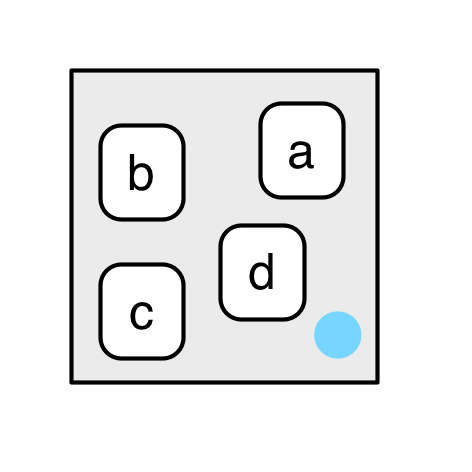
\includegraphics[width=1.18in]{diagrams/environments.png/bag-of-names.png}

Each name points to an object stored elsewhere in memory:

\begin{Shaded}
\begin{Highlighting}[]
\NormalTok{e <-}\StringTok{ }\KeywordTok{new.env}\NormalTok{()}
\NormalTok{e$a <-}\StringTok{ }\OtherTok{FALSE}
\NormalTok{e$b <-}\StringTok{ "a"}
\NormalTok{e$c <-}\StringTok{ }\FloatTok{2.3}
\NormalTok{e$d <-}\StringTok{ }\DecValTok{1}\NormalTok{:}\DecValTok{3}
\end{Highlighting}
\end{Shaded}

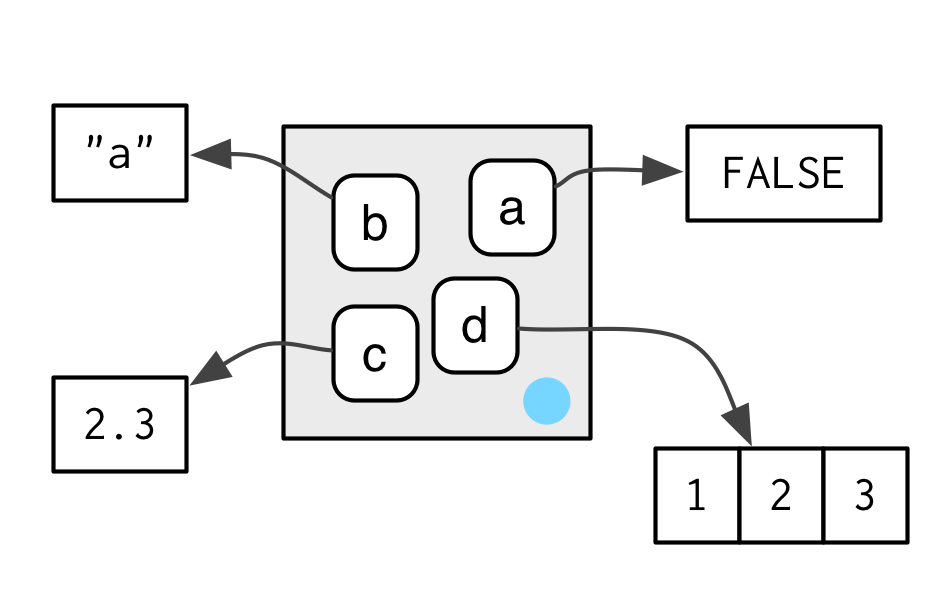
\includegraphics[width=2.36in]{diagrams/environments.png/bindings.png}

The objects don't live in the environment so multiple names can point to
the same object:

\begin{Shaded}
\begin{Highlighting}[]
\NormalTok{e$a <-}\StringTok{ }\NormalTok{e$d}
\end{Highlighting}
\end{Shaded}

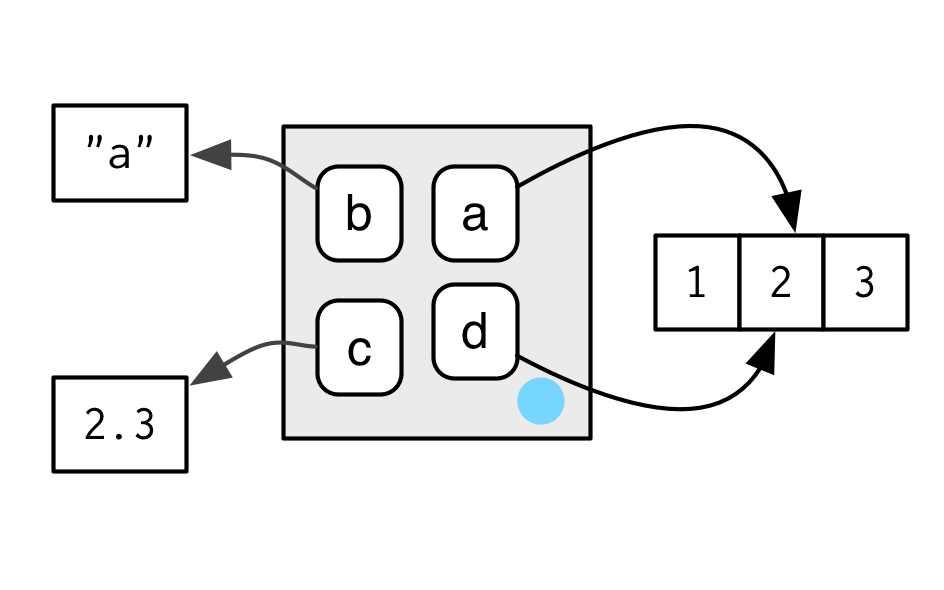
\includegraphics[width=2.36in]{diagrams/environments.png/multiple-names.png}

Confusingly they can also point to different objects that have the same
value:

\begin{Shaded}
\begin{Highlighting}[]
\NormalTok{e$a <-}\StringTok{ }\DecValTok{1}\NormalTok{:}\DecValTok{3}
\end{Highlighting}
\end{Shaded}

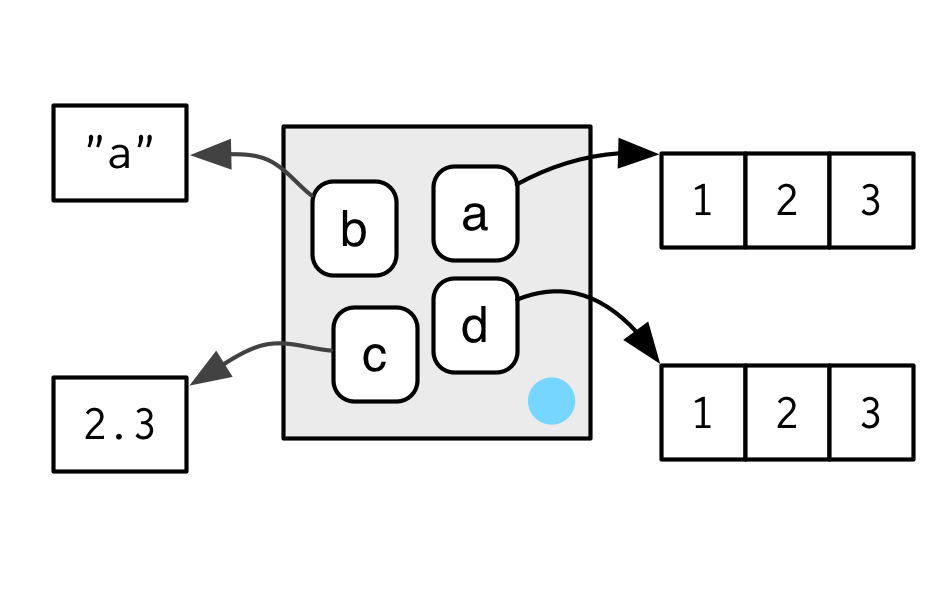
\includegraphics[width=2.36in]{diagrams/environments.png/copies.png}

If an object has no names pointing to it, it gets automatically deleted
by the garbage collector. This process is described in more detail in
\hyperref[gc]{gc}.

Every environment has a parent, another environment. In diagrams, I'll
represent the pointer to parent with a small black circle. The parent is
used to implement lexical scoping: if a name is not found in an
environment, then R will look in its parent (and so on). Only one
environment doesn't have a parent: the \textbf{empty} environment.
\index{environments!empty}

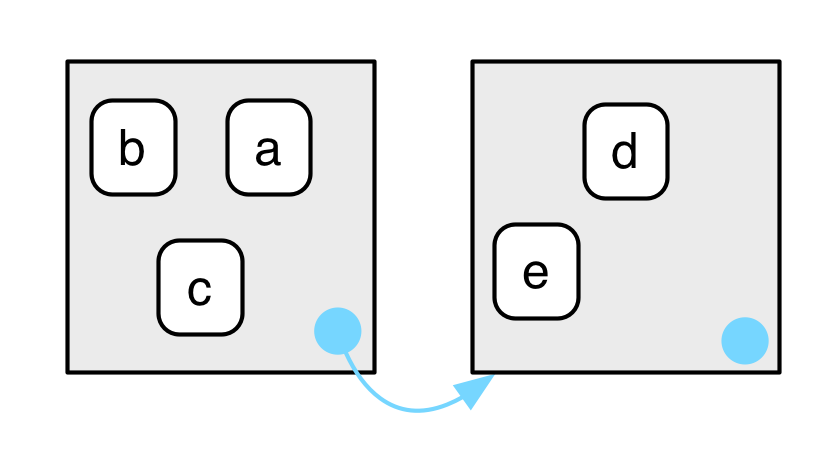
\includegraphics[width=2.36in]{diagrams/environments.png/parents.png}

We use the metaphor of a family to refer to environments. The
grandparent of an environment is the parent's parent, and the ancestors
include all parent environments up to the empty environment. It's rare
to talk about the children of an environment because there are no back
links: given an environment we have no way to find its children.

Generally, an environment is similar to a list, with four important
exceptions:

\begin{itemize}
\item
  Every object in an environment has a unique name.
\item
  The objects in an environment are not ordered (i.e., it doesn't make
  sense to ask what the first object in an environment is).
\item
  An environment has a parent.
\item
  Environments have reference semantics.
\end{itemize}

More technically, an environment is made up of two components, the
\textbf{frame}, which contains the name-object bindings (and behaves
much like a named list), and the parent environment. Unfortunately
``frame'' is used inconsistently in R. For example,
\texttt{parent.frame()} doesn't give you the parent frame of an
environment. Instead, it gives you the \emph{calling} environment. This
is discussed in more detail in \hyperref[calling-environments]{calling
environments}. \index{frames} \index{environments!parent}

There are four special environments:

\begin{itemize}
\item
  The \texttt{globalenv()}, or global environment, is the interactive
  workspace. This is the environment in which you normally work. The
  parent of the global environment is the last package that you attached
  with \texttt{library()} or \texttt{require()}.
\item
  The \texttt{baseenv()}, or base environment, is the environment of the
  base package. Its parent is the empty environment.
\item
  The \texttt{emptyenv()}, or empty environment, is the ultimate
  ancestor of all environments, and the only environment without a
  parent.
\item
  The \texttt{environment()} is the current environment.
\end{itemize}

\texttt{search()} lists all parents of the global environment. This is
called the search path because objects in these environments can be
found from the top-level interactive workspace. It contains one
environment for each attached package and any other objects that you've
\texttt{attach()}ed. It also contains a special environment called
\texttt{Autoloads} which is used to save memory by only loading package
objects (like big datasets) when needed. \indexc{search()}

You can access any environment on the search list using
\texttt{as.environment()}.

\begin{Shaded}
\begin{Highlighting}[]
\KeywordTok{search}\NormalTok{()}
\CommentTok{#> [1] ".GlobalEnv"        "package:stats"     "package:graphics" }
\CommentTok{#> [4] "package:grDevices" "package:utils"     "package:datasets" }
\CommentTok{#> [7] "package:methods"   "Autoloads"         "package:base"     }

\KeywordTok{as.environment}\NormalTok{(}\StringTok{"package:stats"}\NormalTok{)}
\CommentTok{#> <environment: package:stats>}
\end{Highlighting}
\end{Shaded}

\texttt{globalenv()}, \texttt{baseenv()}, the environments on the search
path, and \texttt{emptyenv()} are connected as shown below. Each time
you load a new package with \texttt{library()} it is inserted between
the global environment and the package that was previously at the top of
the search path.

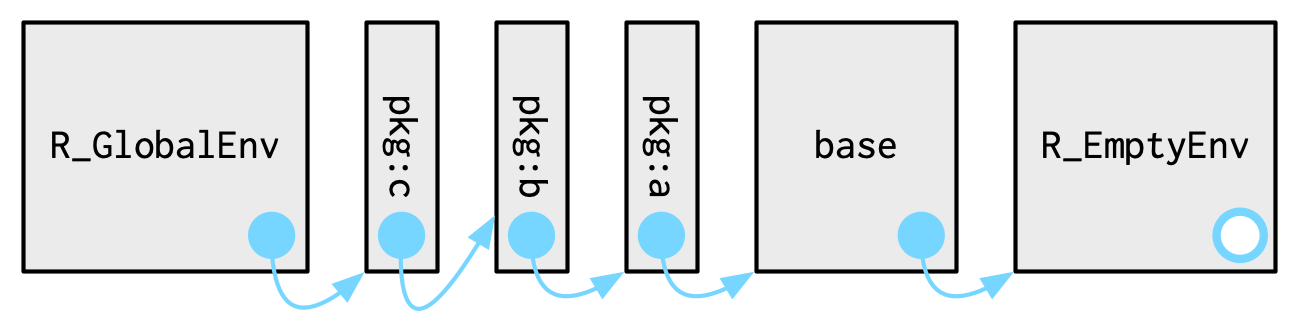
\includegraphics[width=4.35in]{diagrams/environments.png/search-path.png}

To create an environment manually, use \texttt{new.env()}. You can list
the bindings in the environment's frame with \texttt{ls()} and see its
parent with \texttt{parent.env()}. \index{environments!creating}

\begin{Shaded}
\begin{Highlighting}[]
\NormalTok{e <-}\StringTok{ }\KeywordTok{new.env}\NormalTok{()}
\CommentTok{# the default parent provided by new.env() is environment from }
\CommentTok{# which it is called - in this case that's the global environment.}
\KeywordTok{parent.env}\NormalTok{(e)}
\CommentTok{#> <environment: R_GlobalEnv>}
\KeywordTok{ls}\NormalTok{(e)}
\CommentTok{#> character(0)}
\end{Highlighting}
\end{Shaded}

The easiest way to modify the bindings in an environment is to treat it
like a list:

\begin{Shaded}
\begin{Highlighting}[]
\NormalTok{e$a <-}\StringTok{ }\DecValTok{1}
\NormalTok{e$b <-}\StringTok{ }\DecValTok{2}
\KeywordTok{ls}\NormalTok{(e)}
\CommentTok{#> [1] "a" "b"}
\NormalTok{e$a}
\CommentTok{#> [1] 1}
\end{Highlighting}
\end{Shaded}

By default, \texttt{ls()} only shows names that don't begin with
\texttt{.}. Use \texttt{all.names = TRUE} to show all bindings in an
environment: \indexc{ls()}

\begin{Shaded}
\begin{Highlighting}[]
\NormalTok{e$.a <-}\StringTok{ }\DecValTok{2}
\KeywordTok{ls}\NormalTok{(e)}
\CommentTok{#> [1] "a" "b"}
\KeywordTok{ls}\NormalTok{(e, }\DataTypeTok{all.names =} \OtherTok{TRUE}\NormalTok{)}
\CommentTok{#> [1] ".a" "a"  "b"}
\end{Highlighting}
\end{Shaded}

Another useful way to view an environment is \texttt{ls.str()}. It is
more useful than \texttt{str()} because it shows each object in the
environment. Like \texttt{ls()}, it also has an \texttt{all.names}
argument.

\begin{Shaded}
\begin{Highlighting}[]
\KeywordTok{str}\NormalTok{(e)}
\CommentTok{#> <environment: 0x7fba6aac1ad8>}
\KeywordTok{ls.str}\NormalTok{(e)}
\CommentTok{#> a :  num 1}
\CommentTok{#> b :  num 2}
\end{Highlighting}
\end{Shaded}

Given a name, you can extract the value to which it is bound with
\texttt{\$}, \texttt{{[}{[}}, or \texttt{get()}:

\begin{itemize}
\item
  \texttt{\$} and \texttt{{[}{[}} look only in one environment and
  return \texttt{NULL} if there is no binding associated with the name.
  \indexc{\$} \indexc{[[}
\item
  \texttt{get()} uses the regular scoping rules and throws an error if
  the binding is not found. \indexc{get()}
\end{itemize}

\begin{Shaded}
\begin{Highlighting}[]
\NormalTok{e$c <-}\StringTok{ }\DecValTok{3}
\NormalTok{e$c}
\CommentTok{#> [1] 3}
\NormalTok{e[[}\StringTok{"c"}\NormalTok{]]}
\CommentTok{#> [1] 3}
\KeywordTok{get}\NormalTok{(}\StringTok{"c"}\NormalTok{, }\DataTypeTok{envir =} \NormalTok{e)}
\CommentTok{#> [1] 3}
\end{Highlighting}
\end{Shaded}

Deleting objects from environments works a little differently from
lists. With a list you can remove an entry by setting it to
\texttt{NULL}. In environments, that will create a new binding to
\texttt{NULL}. Instead, use \texttt{rm()} to remove the binding.
\indexc{rm()} \index{environments!removing an element}

\begin{Shaded}
\begin{Highlighting}[]
\NormalTok{e <-}\StringTok{ }\KeywordTok{new.env}\NormalTok{()}

\NormalTok{e$a <-}\StringTok{ }\DecValTok{1}
\NormalTok{e$a <-}\StringTok{ }\OtherTok{NULL}
\KeywordTok{ls}\NormalTok{(e)}
\CommentTok{#> [1] "a"}

\KeywordTok{rm}\NormalTok{(}\StringTok{"a"}\NormalTok{, }\DataTypeTok{envir =} \NormalTok{e)}
\KeywordTok{ls}\NormalTok{(e)}
\CommentTok{#> character(0)}
\end{Highlighting}
\end{Shaded}

You can determine if a binding exists in an environment with
\texttt{exists()}. Like \texttt{get()}, its default behaviour is to
follow the regular scoping rules and look in parent environments. If you
don't want this behavior, use \texttt{inherits = FALSE}:

\begin{Shaded}
\begin{Highlighting}[]
\NormalTok{x <-}\StringTok{ }\DecValTok{10}
\KeywordTok{exists}\NormalTok{(}\StringTok{"x"}\NormalTok{, }\DataTypeTok{envir =} \NormalTok{e)}
\CommentTok{#> [1] TRUE}
\KeywordTok{exists}\NormalTok{(}\StringTok{"x"}\NormalTok{, }\DataTypeTok{envir =} \NormalTok{e, }\DataTypeTok{inherits =} \OtherTok{FALSE}\NormalTok{)}
\CommentTok{#> [1] FALSE}
\end{Highlighting}
\end{Shaded}

To compare environments, you must use \texttt{identical()} not
\texttt{==}:

\begin{Shaded}
\begin{Highlighting}[]
\KeywordTok{identical}\NormalTok{(}\KeywordTok{globalenv}\NormalTok{(), }\KeywordTok{environment}\NormalTok{())}
\CommentTok{#> [1] TRUE}
\KeywordTok{globalenv}\NormalTok{() ==}\StringTok{ }\KeywordTok{environment}\NormalTok{()}
\CommentTok{#> Error in globalenv() == environment(): comparison (1) is possible only for atomic and list types}
\end{Highlighting}
\end{Shaded}

\subsection{Exercises}

\begin{enumerate}
\def\labelenumi{\arabic{enumi}.}
\item
  List three ways in which an environment differs from a list.
\item
  If you don't supply an explicit environment, where do \texttt{ls()}
  and \texttt{rm()} look? Where does \texttt{\textless{}-} make
  bindings?
\item
  Using \texttt{parent.env()} and a loop (or a recursive function),
  verify that the ancestors of \texttt{globalenv()} include
  \texttt{baseenv()} and \texttt{emptyenv()}. Use the same basic idea to
  implement your own version of \texttt{search()}.
\end{enumerate}

\hyperdef{}{env-recursion}{\section{Recursing over
environments}\label{env-recursion}}

Environments form a tree, so it's often convenient to write a recursive
function. This section shows you how by applying your new knowledge of
environments to understand the helpful \texttt{pryr::where()}. Given a
name, \texttt{where()} finds the environment \emph{where} that name is
defined, using R's regular scoping rules:
\index{recursion!over environments}

\begin{Shaded}
\begin{Highlighting}[]
\KeywordTok{library}\NormalTok{(pryr)}
\NormalTok{x <-}\StringTok{ }\DecValTok{5}
\KeywordTok{where}\NormalTok{(}\StringTok{"x"}\NormalTok{)}
\CommentTok{#> <environment: R_GlobalEnv>}
\KeywordTok{where}\NormalTok{(}\StringTok{"mean"}\NormalTok{)}
\CommentTok{#> <environment: base>}
\end{Highlighting}
\end{Shaded}

The definition of \texttt{where()} is straightforward. It has two
arguments: the name to look for (as a string), and the environment in
which to start the search. (We'll learn later why
\texttt{parent.frame()} is a good default in
\hyperref[calling-environments]{calling environments}.)

\begin{Shaded}
\begin{Highlighting}[]
\NormalTok{where <-}\StringTok{ }\NormalTok{function(name, }\DataTypeTok{env =} \KeywordTok{parent.frame}\NormalTok{()) \{}
  \NormalTok{if (}\KeywordTok{identical}\NormalTok{(env, }\KeywordTok{emptyenv}\NormalTok{())) \{}
    \CommentTok{# Base case}
    \KeywordTok{stop}\NormalTok{(}\StringTok{"Can't find "}\NormalTok{, name, }\DataTypeTok{call. =} \OtherTok{FALSE}\NormalTok{)}
    
  \NormalTok{\} else if (}\KeywordTok{exists}\NormalTok{(name, }\DataTypeTok{envir =} \NormalTok{env, }\DataTypeTok{inherits =} \OtherTok{FALSE}\NormalTok{)) \{}
    \CommentTok{# Success case}
    \NormalTok{env}
    
  \NormalTok{\} else \{}
    \CommentTok{# Recursive case}
    \KeywordTok{where}\NormalTok{(name, }\KeywordTok{parent.env}\NormalTok{(env))}
    
  \NormalTok{\}}
\NormalTok{\}}
\end{Highlighting}
\end{Shaded}

There are three cases:

\begin{itemize}
\item
  The base case: we've reached the empty environment and haven't found
  the binding. We can't go any further, so we throw an error.
\item
  The successful case: the name exists in this environment, so we return
  the environment.
\item
  The recursive case: the name was not found in this environment, so try
  the parent.
\end{itemize}

It's easier to see what's going on with an example. Imagine you have two
environments as in the following diagram:

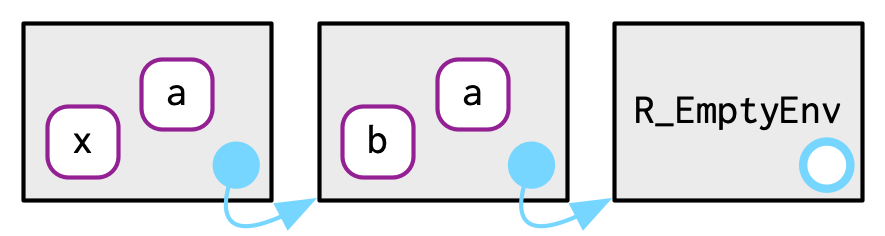
\includegraphics[width=3.32in]{diagrams/environments.png/where-ex.png}

\begin{itemize}
\item
  If you're looking for \texttt{a}, \texttt{where()} will find it in the
  first environment.
\item
  If you're looking for \texttt{b}, it's not in the first environment,
  so \texttt{where()} will look in its parent and find it there.
\item
  If you're looking for \texttt{c}, it's not in the first environment,
  or the second environment, so \texttt{where()} reaches the empty
  environment and throws an error.
\end{itemize}

It's natural to work with environments recursively, so \texttt{where()}
provides a useful template. Removing the specifics of \texttt{where()}
shows the structure more clearly:

\begin{Shaded}
\begin{Highlighting}[]
\NormalTok{f <-}\StringTok{ }\NormalTok{function(..., }\DataTypeTok{env =} \KeywordTok{parent.frame}\NormalTok{()) \{}
  \NormalTok{if (}\KeywordTok{identical}\NormalTok{(env, }\KeywordTok{emptyenv}\NormalTok{())) \{}
    \CommentTok{# base case}
  \NormalTok{\} else if (success) \{}
    \CommentTok{# success case}
  \NormalTok{\} else \{}
    \CommentTok{# recursive case}
    \KeywordTok{f}\NormalTok{(..., }\DataTypeTok{env =} \KeywordTok{parent.env}\NormalTok{(env))}
  \NormalTok{\}}
\NormalTok{\}}
\end{Highlighting}
\end{Shaded}

\begin{shortbox}\Boxhead{Iteration vs. recursion}

It's possible to use a loop instead of recursion. This might run
slightly faster (because we eliminate some function calls), but I think
it's harder to understand. I include it because you might find it easier
to see what's happening if you're less familiar with recursive
functions.

\begin{Shaded}
\begin{Highlighting}[]
\NormalTok{is_empty <-}\StringTok{ }\NormalTok{function(x) }\KeywordTok{identical}\NormalTok{(x, }\KeywordTok{emptyenv}\NormalTok{())}

\NormalTok{f2 <-}\StringTok{ }\NormalTok{function(..., }\DataTypeTok{env =} \KeywordTok{parent.frame}\NormalTok{()) \{}
  \NormalTok{while(!}\KeywordTok{is_empty}\NormalTok{(env)) \{}
    \NormalTok{if (success) \{}
      \CommentTok{# success case}
      \KeywordTok{return}\NormalTok{()}
    \NormalTok{\}}
    \CommentTok{# inspect parent}
    \NormalTok{env <-}\StringTok{ }\KeywordTok{parent.env}\NormalTok{(env)}
  \NormalTok{\}}

  \CommentTok{# base case}
\NormalTok{\}}
\end{Highlighting}
\end{Shaded}

\end{shortbox}

\subsection{Exercises}

\begin{enumerate}
\def\labelenumi{\arabic{enumi}.}
\item
  Modify \texttt{where()} to find all environments that contain a
  binding for \texttt{name}.
\item
  Write your own version of \texttt{get()} using a function written in
  the style of \texttt{where()}.
\item
  Write a function called \texttt{fget()} that finds only function
  objects. It should have two arguments, \texttt{name} and \texttt{env},
  and should obey the regular scoping rules for functions: if there's an
  object with a matching name that's not a function, look in the parent.
  For an added challenge, also add an \texttt{inherits} argument which
  controls whether the function recurses up the parents or only looks in
  one environment.
\item
  Write your own version of \texttt{exists(inherits = FALSE)} (Hint: use
  \texttt{ls()}.) Write a recursive version that behaves like
  \texttt{exists(inherits = TRUE)}.
\end{enumerate}

\hyperdef{}{function-envs}{\section{Function
environments}\label{function-envs}}

Most environments are not created by you with \texttt{new.env()} but are
created as a consequence of using functions. This section discusses the
four types of environments associated with a function: enclosing,
binding, execution, and calling. \index{functions!environments}

The \textbf{enclosing} environment is the environment where the function
was created. Every function has one and only one enclosing environment.
For the three other types of environment, there may be 0, 1, or many
environments associated with each function:

\begin{itemize}
\item
  Binding a function to a name with \texttt{\textless{}-} defines a
  \textbf{binding} environment.
\item
  Calling a function creates an ephemeral \textbf{execution} environment
  that stores variables created during execution.
\item
  Every execution environment is associated with a \textbf{calling}
  environment, which tells you where the function was called.
\end{itemize}

The following sections will explain why each of these environments is
important, how to access them, and how you might use them.

\subsection{The enclosing environment}

When a function is created, it gains a reference to the environment
where it was made. This is the \textbf{enclosing environment} and is
used for lexical scoping. You can determine the enclosing environment of
a function by calling \texttt{environment()} with a function as its
first argument: \index{environments!enclosing}

\begin{Shaded}
\begin{Highlighting}[]
\NormalTok{y <-}\StringTok{ }\DecValTok{1}
\NormalTok{f <-}\StringTok{ }\NormalTok{function(x) x +}\StringTok{ }\NormalTok{y}
\KeywordTok{environment}\NormalTok{(f)}
\CommentTok{#> <environment: R_GlobalEnv>}
\end{Highlighting}
\end{Shaded}

In diagrams, I'll depict functions as rounded rectangles. The enclosing
environment of a function is given by a small black circle:

\includegraphics[width=2.06in]{diagrams/environments.png/enclosing.png}

\subsection{Binding environments}

The previous diagram is too simple because functions don't have names.
Instead, the name of a function is defined by a binding. The binding
environments of a function are all the environments which have a binding
to it. The following diagram better reflects this relationship because
the enclosing environment contains a binding from \texttt{f} to the
function: \index{environments!binding names}

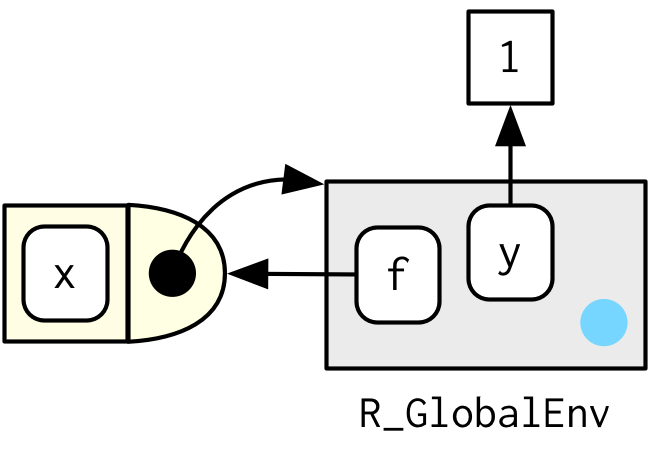
\includegraphics[width=2.06in]{diagrams/environments.png/binding.png}

In this case the enclosing and binding environments are the same. They
will be different if you assign a function into a different environment:

\begin{Shaded}
\begin{Highlighting}[]
\NormalTok{e <-}\StringTok{ }\KeywordTok{new.env}\NormalTok{()}
\NormalTok{e$g <-}\StringTok{ }\NormalTok{function() }\DecValTok{1}
\end{Highlighting}
\end{Shaded}

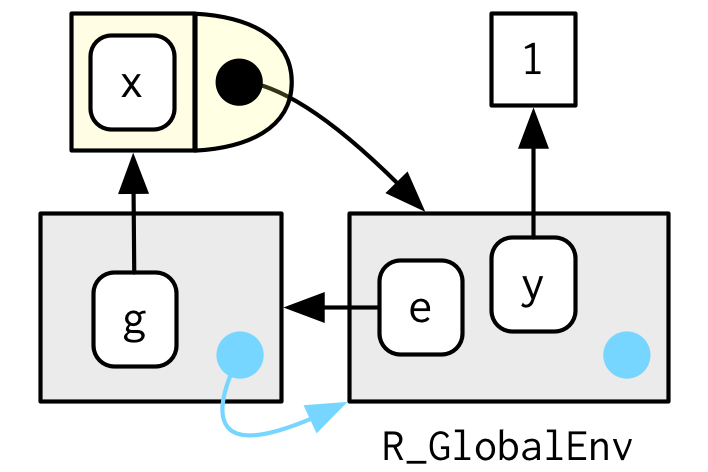
\includegraphics[width=2.06in]{diagrams/environments.png/binding-2.png}

The enclosing environment belongs to the function, and never changes,
even if the function is moved to a different environment. The enclosing
environment determines how the function finds values; the binding
environments determine how we find the function.

The distinction between the binding environment and the enclosing
environment is important for package namespaces. Package namespaces keep
packages independent. For example, if package A uses the base
\texttt{mean()} function, what happens if package B creates its own
\texttt{mean()} function? Namespaces ensure that package A continues to
use the base \texttt{mean()} function, and that package A is not
affected by package B (unless explicitly asked for). \index{namespaces}

Namespaces are implemented using environments, taking advantage of the
fact that functions don't have to live in their enclosing environments.
For example, take the base function \texttt{sd()}. It's binding and
enclosing environments are different:

\begin{Shaded}
\begin{Highlighting}[]
\KeywordTok{environment}\NormalTok{(sd)}
\CommentTok{#> <environment: namespace:stats>}
\KeywordTok{where}\NormalTok{(}\StringTok{"sd"}\NormalTok{)}
\CommentTok{#> <environment: package:stats>}
\end{Highlighting}
\end{Shaded}

The definition of \texttt{sd()} uses \texttt{var()}, but if we make our
own version of \texttt{var()} it doesn't affect \texttt{sd()}:

\begin{Shaded}
\begin{Highlighting}[]
\NormalTok{x <-}\StringTok{ }\DecValTok{1}\NormalTok{:}\DecValTok{10}
\KeywordTok{sd}\NormalTok{(x)}
\CommentTok{#> [1] 3.03}
\NormalTok{var <-}\StringTok{ }\NormalTok{function(x, }\DataTypeTok{na.rm =} \OtherTok{TRUE}\NormalTok{) }\DecValTok{100}
\KeywordTok{sd}\NormalTok{(x)}
\CommentTok{#> [1] 3.03}
\end{Highlighting}
\end{Shaded}

This works because every package has two environments associated with
it: the \emph{package} environment and the \emph{namespace} environment.
The package environment contains every publicly accessible function, and
is placed on the search path. The namespace environment contains all
functions (including internal functions), and its parent environment is
a special imports environment that contains bindings to all the
functions that the package needs. Every exported function in a package
is bound into the \emph{package} environment, but enclosed by the
\emph{namespace} environment. This complicated relationship is
illustrated by the following diagram:

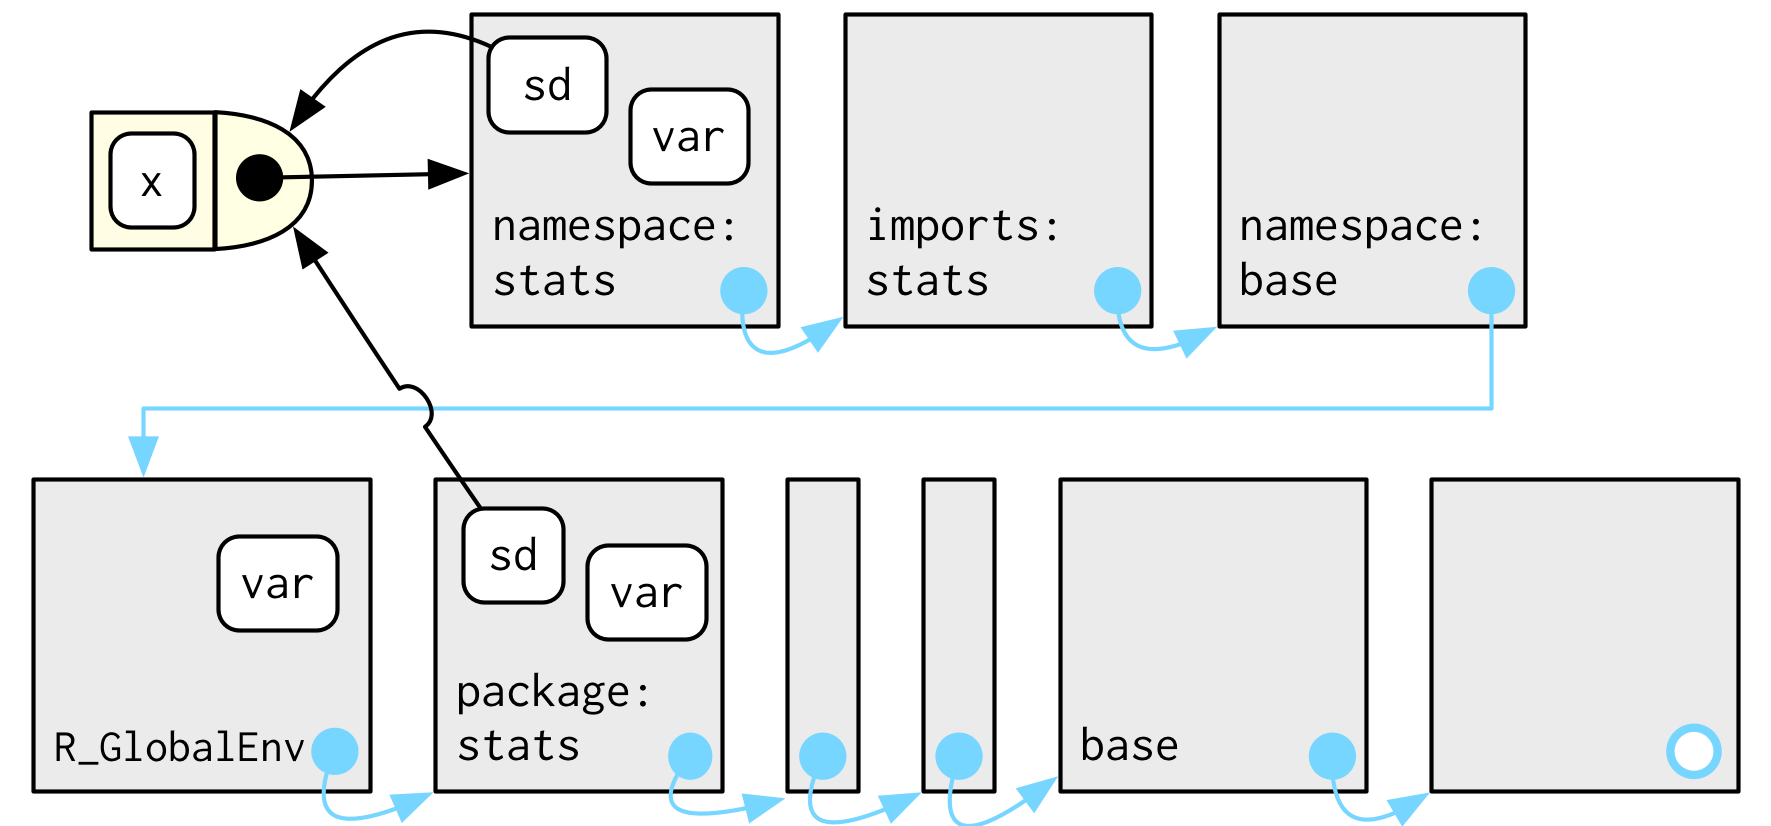
\includegraphics[width=4.35in]{diagrams/environments.png/namespace.png}

When we type \texttt{var} into the console, it's found first in the
global environment. When \texttt{sd()} looks for \texttt{var()} it finds
it first in its namespace environment so never looks in the
\texttt{globalenv()}.

\subsection{Execution environments}

What will the following function return the first time it's run? What
about the second? \index{environments!execution}

\begin{Shaded}
\begin{Highlighting}[]
\NormalTok{g <-}\StringTok{ }\NormalTok{function(x) \{}
  \NormalTok{if (!}\KeywordTok{exists}\NormalTok{(}\StringTok{"a"}\NormalTok{, }\DataTypeTok{inherits =} \OtherTok{FALSE}\NormalTok{)) \{}
    \KeywordTok{message}\NormalTok{(}\StringTok{"Defining a"}\NormalTok{)}
    \NormalTok{a <-}\StringTok{ }\DecValTok{1}
  \NormalTok{\} else \{}
    \NormalTok{a <-}\StringTok{ }\NormalTok{a +}\StringTok{ }\DecValTok{1}
  \NormalTok{\}}
  \NormalTok{a}
\NormalTok{\}}
\KeywordTok{g}\NormalTok{(}\DecValTok{10}\NormalTok{)}
\KeywordTok{g}\NormalTok{(}\DecValTok{10}\NormalTok{)}
\end{Highlighting}
\end{Shaded}

This function returns the same value every time it is called because of
the fresh start principle, described in \hyperref[fresh-start]{a fresh
start}. Each time a function is called, a new environment is created to
host execution. The parent of the execution environment is the enclosing
environment of the function. Once the function has completed, this
environment is thrown away.

Let's depict that graphically with a simpler function. I draw execution
environments around the function they belong to with a dotted border.

\begin{Shaded}
\begin{Highlighting}[]
\NormalTok{h <-}\StringTok{ }\NormalTok{function(x) \{}
  \NormalTok{a <-}\StringTok{ }\DecValTok{2}
  \NormalTok{x +}\StringTok{ }\NormalTok{a}
\NormalTok{\}}
\NormalTok{y <-}\StringTok{ }\KeywordTok{h}\NormalTok{(}\DecValTok{1}\NormalTok{)}
\end{Highlighting}
\end{Shaded}

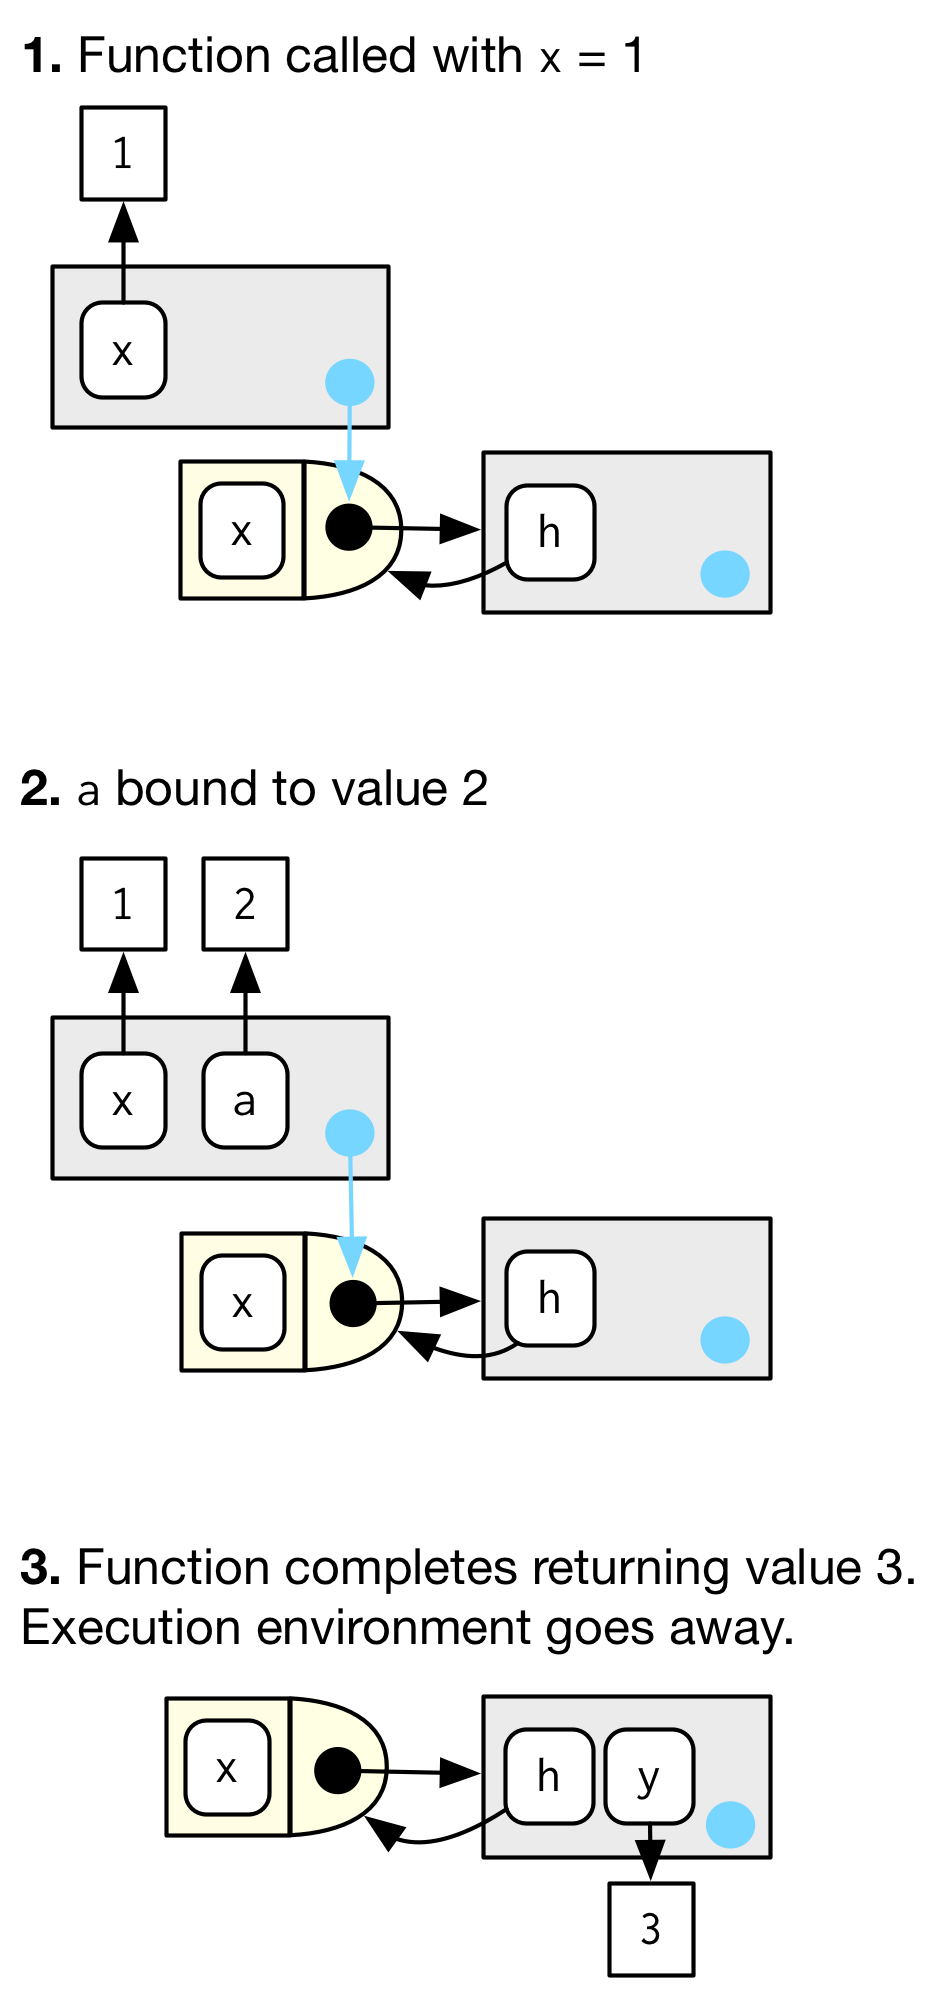
\includegraphics[width=2.95in]{diagrams/environments.png/execution.png}

When you create a function inside another function, the enclosing
environment of the child function is the execution environment of the
parent, and the execution environment is no longer ephemeral. The
following example illustrates that idea with a function factory,
\texttt{plus()}. We use that factory to create a function called
\texttt{plus\_one()}. The enclosing environment of \texttt{plus\_one()}
is the execution environment of \texttt{plus()} where \texttt{x} is
bound to the value 1. \index{closures|environment}

\begin{Shaded}
\begin{Highlighting}[]
\NormalTok{plus <-}\StringTok{ }\NormalTok{function(x) \{}
  \NormalTok{function(y) x +}\StringTok{ }\NormalTok{y}
\NormalTok{\}}
\NormalTok{plus_one <-}\StringTok{ }\KeywordTok{plus}\NormalTok{(}\DecValTok{1}\NormalTok{)}
\KeywordTok{identical}\NormalTok{(}\KeywordTok{parent.env}\NormalTok{(}\KeywordTok{environment}\NormalTok{(plus_one)), }\KeywordTok{environment}\NormalTok{(plus))}
\CommentTok{#> [1] TRUE}
\end{Highlighting}
\end{Shaded}

\includegraphics[width=2.51in]{diagrams/environments.png/closure-2.png}

You'll learn more about function factories in
\hyperref[functional-programming]{functional programming}.

\hyperdef{}{calling-environments}{\subsection{Calling
environments}\label{calling-environments}}

Look at the following code. What do you expect \texttt{i()} to return
when the code is run? \index{environments|calling}

\begin{Shaded}
\begin{Highlighting}[]
\NormalTok{h <-}\StringTok{ }\NormalTok{function() \{}
  \NormalTok{x <-}\StringTok{ }\DecValTok{10}
  \NormalTok{function() \{}
    \NormalTok{x}
  \NormalTok{\}}
\NormalTok{\}}
\NormalTok{i <-}\StringTok{ }\KeywordTok{h}\NormalTok{()}
\NormalTok{x <-}\StringTok{ }\DecValTok{20}
\KeywordTok{i}\NormalTok{()}
\end{Highlighting}
\end{Shaded}

The top-level \texttt{x} (bound to 20) is a red herring: using the
regular scoping rules, \texttt{h()} looks first where it is defined and
finds that the value associated with \texttt{x} is 10. However, it's
still meaningful to ask what value \texttt{x} is associated within the
environment where \texttt{i()} is called: \texttt{x} is 10 in the
environment where \texttt{h()} is defined, but it is 20 in the
environment where \texttt{h()} is called.

We can access this environment using the unfortunately named
\texttt{parent.frame()}. This function returns the \textbf{environment}
where the function was called. We can also use this function to look up
the value of names in that environment:

\begin{Shaded}
\begin{Highlighting}[]
\NormalTok{f2 <-}\StringTok{ }\NormalTok{function() \{}
  \NormalTok{x <-}\StringTok{ }\DecValTok{10}
  \NormalTok{function() \{}
    \NormalTok{def <-}\StringTok{ }\KeywordTok{get}\NormalTok{(}\StringTok{"x"}\NormalTok{, }\KeywordTok{environment}\NormalTok{())}
    \NormalTok{cll <-}\StringTok{ }\KeywordTok{get}\NormalTok{(}\StringTok{"x"}\NormalTok{, }\KeywordTok{parent.frame}\NormalTok{())}
    \KeywordTok{list}\NormalTok{(}\DataTypeTok{defined =} \NormalTok{def, }\DataTypeTok{called =} \NormalTok{cll)}
  \NormalTok{\}}
\NormalTok{\}}
\NormalTok{g2 <-}\StringTok{ }\KeywordTok{f2}\NormalTok{()}
\NormalTok{x <-}\StringTok{ }\DecValTok{20}
\KeywordTok{str}\NormalTok{(}\KeywordTok{g2}\NormalTok{())}
\CommentTok{#> List of 2}
\CommentTok{#>  $ defined: num 10}
\CommentTok{#>  $ called : num 20}
\end{Highlighting}
\end{Shaded}

In more complicated scenarios, there's not just one parent call, but a
sequence of calls which lead all the way back to the initiating
function, called from the top-level. The following code generates a call
stack three levels deep. The open-ended arrows represent the calling
environment of each execution environment.

\begin{Shaded}
\begin{Highlighting}[]
\NormalTok{x <-}\StringTok{ }\DecValTok{0}
\NormalTok{y <-}\StringTok{ }\DecValTok{10}
\NormalTok{f <-}\StringTok{ }\NormalTok{function() \{}
  \NormalTok{x <-}\StringTok{ }\DecValTok{1}
  \KeywordTok{g}\NormalTok{()}
\NormalTok{\}}
\NormalTok{g <-}\StringTok{ }\NormalTok{function() \{}
  \NormalTok{x <-}\StringTok{ }\DecValTok{2}
  \KeywordTok{h}\NormalTok{()}
\NormalTok{\}}
\NormalTok{h <-}\StringTok{ }\NormalTok{function() \{}
  \NormalTok{x <-}\StringTok{ }\DecValTok{3}
  \NormalTok{x +}\StringTok{ }\NormalTok{y}
\NormalTok{\}}
\KeywordTok{f}\NormalTok{()}
\CommentTok{#> [1] 13}
\end{Highlighting}
\end{Shaded}

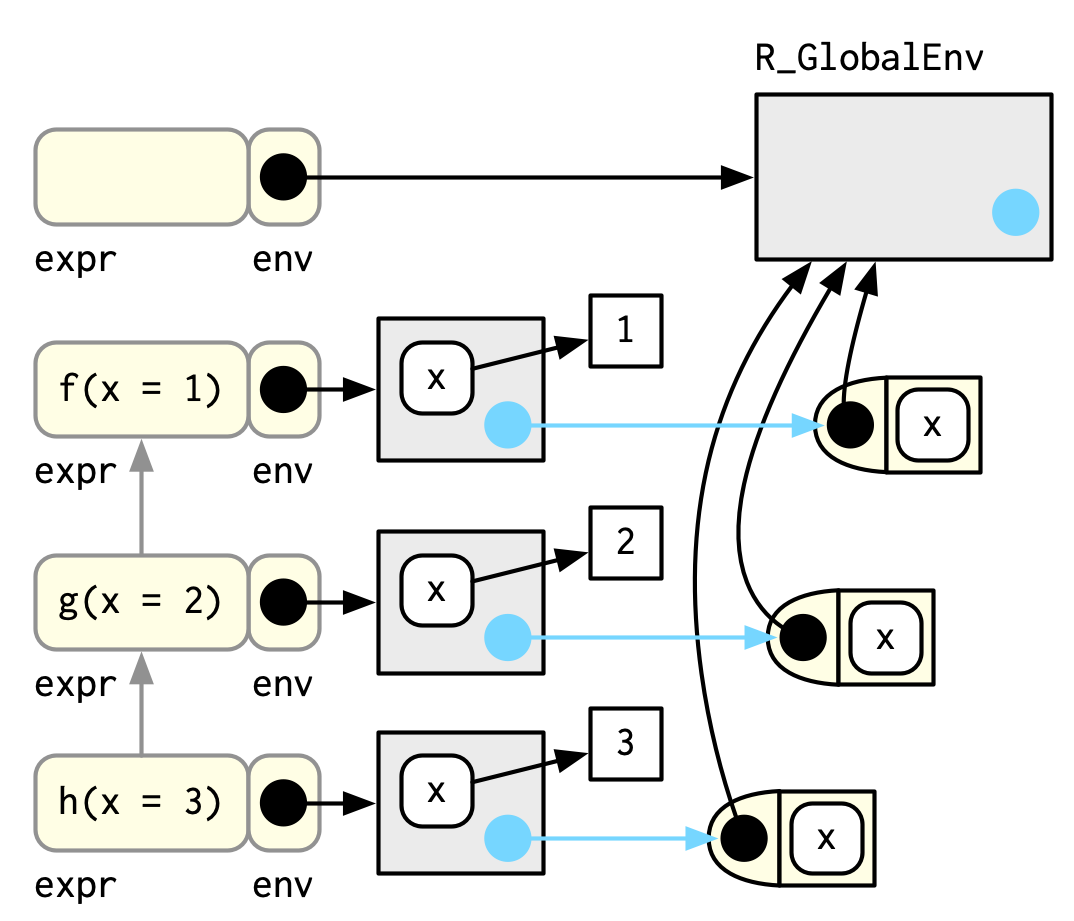
\includegraphics[width=3.25in]{diagrams/environments.png/calling.png}

Note that each execution environment has two parents: a calling
environment and an enclosing environment. R's regular scoping rules only
use the enclosing parent; \texttt{parent.frame()} allows you to access
the calling parent.

Looking up variables in the calling environment rather than in the
enclosing environment is called \textbf{dynamic scoping}. Few languages
implement dynamic scoping (Emacs Lisp is a
\href{http://www.gnu.org/software/emacs/emacs-paper.html\#SEC15}{notable
exception}.) This is because dynamic scoping makes it much harder to
reason about how a function operates: not only do you need to know how
it was defined, you also need to know in what context it was called.
Dynamic scoping is primarily useful for developing functions that aid
interactive data analysis. It is one of the topics discussed in
\hyperref[nse]{non-standard evaluation}. \index{scoping!dynamic}
\index{dynamic scoping}

\subsection{Exercises}

\begin{enumerate}
\def\labelenumi{\arabic{enumi}.}
\item
  List the four environments associated with a function. What does each
  one do? Why is the distinction between enclosing and binding
  environments particularly important?
\item
  Draw a diagram that shows the enclosing environments of this function:

\begin{Shaded}
\begin{Highlighting}[]
\NormalTok{f1 <-}\StringTok{ }\NormalTok{function(x1) \{}
  \NormalTok{f2 <-}\StringTok{ }\NormalTok{function(x2) \{}
    \NormalTok{f3 <-}\StringTok{ }\NormalTok{function(x3) \{}
      \NormalTok{x1 +}\StringTok{ }\NormalTok{x2 +}\StringTok{ }\NormalTok{x3}
    \NormalTok{\}}
    \KeywordTok{f3}\NormalTok{(}\DecValTok{3}\NormalTok{)}
  \NormalTok{\}}
  \KeywordTok{f2}\NormalTok{(}\DecValTok{2}\NormalTok{)}
\NormalTok{\}}
\KeywordTok{f1}\NormalTok{(}\DecValTok{1}\NormalTok{)}
\end{Highlighting}
\end{Shaded}
\item
  Expand your previous diagram to show function bindings.
\item
  Expand it again to show the execution and calling environments.
\item
  Write an enhanced version of \texttt{str()} that provides more
  information about functions. Show where the function was found and
  what environment it was defined in.
\end{enumerate}

\hyperdef{}{binding}{\section{Binding names to values}\label{binding}}

Assignment is the act of binding (or rebinding) a name to a value in an
environment. It is the counterpart to scoping, the set of rules that
determines how to find the value associated with a name. Compared to
most languages, R has extremely flexible tools for binding names to
values. In fact, you can not only bind values to names, but you can also
bind expressions (promises) or even functions, so that every time you
access the value associated with a name, you get something different!
\index{bindings}

You've probably used regular assignment in R thousands of times. Regular
assignment creates a binding between a name and an object in the current
environment. Names usually consist of letters, digits, \texttt{.} and
\texttt{\_}, and can't begin with \texttt{\_}. If you try to use a name
that doesn't follow these rules, you get an error:

\begin{Shaded}
\begin{Highlighting}[]
\NormalTok{_abc <-}\StringTok{ }\DecValTok{1}
\CommentTok{# Error: unexpected input in "_"}
\end{Highlighting}
\end{Shaded}

Reserved words (like \texttt{TRUE}, \texttt{NULL}, \texttt{if}, and
\texttt{function}) follow the rules but are reserved by R for other
purposes:

\begin{Shaded}
\begin{Highlighting}[]
\NormalTok{if <-}\StringTok{ }\DecValTok{10}
\CommentTok{#> Error: unexpected assignment in "if <-"}
\end{Highlighting}
\end{Shaded}

A complete list of reserved words can be found in \texttt{?Reserved}.
\index{reserved names} \indexc{`} \index{non-syntactic names}

It's possible to override the usual rules and use a name with any
sequence of characters by surrounding the name with backticks:

\begin{Shaded}
\begin{Highlighting}[]
\StringTok{`}\DataTypeTok{a + b}\StringTok{`} \NormalTok{<-}\StringTok{ }\DecValTok{3}
\StringTok{`}\DataTypeTok{:)}\StringTok{`} \NormalTok{<-}\StringTok{ "smile"}
\StringTok{`}\DataTypeTok{    }\StringTok{`} \NormalTok{<-}\StringTok{ "spaces"}
\KeywordTok{ls}\NormalTok{()}
\CommentTok{#  [1] "    "   ":)"     "a + b"}
\StringTok{`}\DataTypeTok{:)}\StringTok{`}
\CommentTok{#  [1] "smile"}
\end{Highlighting}
\end{Shaded}

\begin{shortbox}\Boxhead{Quotes}

You can also create non-syntactic bindings using single and double
quotes instead of backticks, but I don't recommend it. The ability to
use strings on the left hand side of the assignment arrow is a
historical artefact, used before R supported backticks.

\end{shortbox}

The regular assignment arrow, \texttt{\textless{}-}, always creates a
variable in the current environment. The deep assignment arrow,
\texttt{\textless{}\textless{}-}, never creates a variable in the
current environment, but instead modifies an existing variable found by
walking up the parent environments. You can also do deep binding with
\texttt{assign()}: \texttt{name \textless{}\textless{}- value} is
equivalent to \texttt{assign("name", value, inherits = TRUE)}.

\begin{Shaded}
\begin{Highlighting}[]
\NormalTok{x <-}\StringTok{ }\DecValTok{0}
\NormalTok{f <-}\StringTok{ }\NormalTok{function() \{}
  \NormalTok{x <<-}\StringTok{ }\DecValTok{1}
\NormalTok{\}}
\KeywordTok{f}\NormalTok{()}
\NormalTok{x}
\CommentTok{#> [1] 1}
\end{Highlighting}
\end{Shaded}

If \texttt{\textless{}\textless{}-} doesn't find an existing variable,
it will create one in the global environment. This is usually
undesirable, because global variables introduce non-obvious dependencies
between functions. \texttt{\textless{}\textless{}-} is most often used
in conjunction with a closure, as described in
\hyperref[closures]{Closures}.

There are two other special types of binding, delayed and active:

\begin{itemize}
\item
  Rather than assigning the result of an expression immediately, a
  \textbf{delayed binding} creates and stores a promise to evaluate the
  expression when needed. We can create delayed bindings with the
  special assignment operator \texttt{\%\textless{}d-\%}, provided by
  the pryr package.

\begin{Shaded}
\begin{Highlighting}[]
\KeywordTok{library}\NormalTok{(pryr)}
\KeywordTok{system.time}\NormalTok{(b %<d-%}\StringTok{ }\NormalTok{\{}\KeywordTok{Sys.sleep}\NormalTok{(}\DecValTok{1}\NormalTok{); }\DecValTok{1}\NormalTok{\})}
\CommentTok{#>    user  system elapsed }
\CommentTok{#>   0.000   0.000   0.001}
\KeywordTok{system.time}\NormalTok{(b)}
\CommentTok{#>    user  system elapsed }
\CommentTok{#>   0.000   0.000   1.001}
\end{Highlighting}
\end{Shaded}

  \texttt{\%\textless{}d-\%} is a wrapper around the base
  \texttt{delayedAssign()} function, which you may need to use directly
  if you need more control. Delayed bindings are used to implement
  \texttt{autoload()}, which makes R behave as if the package data is in
  memory, even though it's only loaded from disk when you ask for it.
  \index{bindings!delayed}
\item
  \textbf{Active} are not bound to a constant object. Instead, they're
  re-computed every time they're accessed:

\begin{Shaded}
\begin{Highlighting}[]
\NormalTok{x %<a-%}\StringTok{ }\KeywordTok{runif}\NormalTok{(}\DecValTok{1}\NormalTok{)}
\NormalTok{x}
\CommentTok{#> [1] 0.0808}
\NormalTok{x}
\CommentTok{#> [1] 0.834}
\KeywordTok{rm}\NormalTok{(x)}
\end{Highlighting}
\end{Shaded}

  \texttt{\%\textless{}a-\%} is a wrapper for the base function
  \texttt{makeActiveBinding()}. You may want to use this function
  directly if you want more control. Active bindings are used to
  implement reference class fields. \index{bindings!active}
\end{itemize}

\subsection{Exercises}

\begin{enumerate}
\def\labelenumi{\arabic{enumi}.}
\item
  What does this function do? How does it differ from
  \texttt{\textless{}\textless{}-} and why might you prefer it?

\begin{Shaded}
\begin{Highlighting}[]
\NormalTok{rebind <-}\StringTok{ }\NormalTok{function(name, value, }\DataTypeTok{env =} \KeywordTok{parent.frame}\NormalTok{()) \{}
  \NormalTok{if (}\KeywordTok{identical}\NormalTok{(env, }\KeywordTok{emptyenv}\NormalTok{())) \{}
    \KeywordTok{stop}\NormalTok{(}\StringTok{"Can't find "}\NormalTok{, name, }\DataTypeTok{call. =} \OtherTok{FALSE}\NormalTok{)}
  \NormalTok{\} else if (}\KeywordTok{exists}\NormalTok{(name, }\DataTypeTok{envir =} \NormalTok{env, }\DataTypeTok{inherits =} \OtherTok{FALSE}\NormalTok{)) \{}
    \KeywordTok{assign}\NormalTok{(name, value, }\DataTypeTok{envir =} \NormalTok{env)}
  \NormalTok{\} else \{}
    \KeywordTok{rebind}\NormalTok{(name, value, }\KeywordTok{parent.env}\NormalTok{(env))}
  \NormalTok{\}}
\NormalTok{\}}
\KeywordTok{rebind}\NormalTok{(}\StringTok{"a"}\NormalTok{, }\DecValTok{10}\NormalTok{)}
\CommentTok{#> Error: Can't find a}
\NormalTok{a <-}\StringTok{ }\DecValTok{5}
\KeywordTok{rebind}\NormalTok{(}\StringTok{"a"}\NormalTok{, }\DecValTok{10}\NormalTok{)}
\NormalTok{a}
\CommentTok{#> [1] 10}
\end{Highlighting}
\end{Shaded}
\item
  Create a version of \texttt{assign()} that will only bind new names,
  never re-bind old names. Some programming languages only do this, and
  are known as
  \href{http://en.wikipedia.org/wiki/Assignment_(computer_science)\#Single_assignment}{single
  assignment languages}.
\item
  Write an assignment function that can do active, delayed, and locked
  bindings. What might you call it? What arguments should it take? Can
  you guess which sort of assignment it should do based on the input?
\end{enumerate}

\hyperdef{}{explicit-envs}{\section{Explicit
environments}\label{explicit-envs}}

As well as powering scoping, environments are also useful data
structures in their own right because they have \textbf{reference
semantics}. Unlike most objects in R, when you modify an environment, it
does not make a copy. For example, look at this \texttt{modify()}
function. \index{copy-on-modify!exceptions} \index{reference semantics}

\begin{Shaded}
\begin{Highlighting}[]
\NormalTok{modify <-}\StringTok{ }\NormalTok{function(x) \{}
  \NormalTok{x$a <-}\StringTok{ }\DecValTok{2}
  \KeywordTok{invisible}\NormalTok{()}
\NormalTok{\}}
\end{Highlighting}
\end{Shaded}

If you apply it to a list, the original list is not changed because
modifying a list actually creates and modifies a copy.

\begin{Shaded}
\begin{Highlighting}[]
\NormalTok{x_l <-}\StringTok{ }\KeywordTok{list}\NormalTok{()}
\NormalTok{x_l$a <-}\StringTok{ }\DecValTok{1}
\KeywordTok{modify}\NormalTok{(x_l)}
\NormalTok{x_l$a}
\CommentTok{#> [1] 1}
\end{Highlighting}
\end{Shaded}

However, if you apply it to an environment, the original environment
\emph{is} modified:

\begin{Shaded}
\begin{Highlighting}[]
\NormalTok{x_e <-}\StringTok{ }\KeywordTok{new.env}\NormalTok{()}
\NormalTok{x_e$a <-}\StringTok{ }\DecValTok{1}
\KeywordTok{modify}\NormalTok{(x_e)}
\NormalTok{x_e$a}
\CommentTok{#> [1] 2}
\end{Highlighting}
\end{Shaded}

Just as you can use a list to pass data between functions, you can also
use an environment. When creating your own environment, note that you
should set its parent environment to be the empty environment. This
ensures you don't accidentally inherit objects from somewhere else:

\begin{Shaded}
\begin{Highlighting}[]
\NormalTok{x <-}\StringTok{ }\DecValTok{1}
\NormalTok{e1 <-}\StringTok{ }\KeywordTok{new.env}\NormalTok{()}
\KeywordTok{get}\NormalTok{(}\StringTok{"x"}\NormalTok{, }\DataTypeTok{envir =} \NormalTok{e1)}
\CommentTok{#> [1] 1}

\NormalTok{e2 <-}\StringTok{ }\KeywordTok{new.env}\NormalTok{(}\DataTypeTok{parent =} \KeywordTok{emptyenv}\NormalTok{())}
\KeywordTok{get}\NormalTok{(}\StringTok{"x"}\NormalTok{, }\DataTypeTok{envir =} \NormalTok{e2)}
\CommentTok{#> Error in get("x", envir = e2): object 'x' not found}
\end{Highlighting}
\end{Shaded}

Environments are data structures useful for solving three common
problems:

\begin{itemize}
\itemsep1pt\parskip0pt\parsep0pt
\item
  Avoiding copies of large data.
\item
  Managing state within a package.
\item
  Efficiently looking up values from names.
\end{itemize}

These are described in turn below.

\subsection{Avoiding copies}

Since environments have reference semantics, you'll never accidentally
create a copy. This makes it a useful vessel for large objects. It's a
common technique for bioconductor packages which often have to manage
large genomic objects. Changes to R 3.1.0 have made this use
substantially less important because modifying a list no longer makes a
deep copy. Previously, modifying a single element of a list would cause
every element to be copied, an expensive operation if some elements are
large. Now, modifying a list efficiently reuses existing vectors, saving
much time.

\subsection{Package state}

Explicit environments are useful in packages because they allow you to
maintain state across function calls. Normally, objects in a package are
locked, so you can't modify them directly. Instead, you can do something
like this:

\begin{Shaded}
\begin{Highlighting}[]
\NormalTok{my_env <-}\StringTok{ }\KeywordTok{new.env}\NormalTok{(}\DataTypeTok{parent =} \KeywordTok{emptyenv}\NormalTok{())}
\NormalTok{my_env$a <-}\StringTok{ }\DecValTok{1}

\NormalTok{get_a <-}\StringTok{ }\NormalTok{function() \{}
  \NormalTok{my_env$a}
\NormalTok{\}}
\NormalTok{set_a <-}\StringTok{ }\NormalTok{function(value) \{}
  \NormalTok{old <-}\StringTok{ }\NormalTok{my_env$a}
  \NormalTok{my_env$a <-}\StringTok{ }\NormalTok{value}
  \KeywordTok{invisible}\NormalTok{(old)}
\NormalTok{\}}
\end{Highlighting}
\end{Shaded}

Returning the old value from setter functions is a good pattern because
it makes it easier to reset the previous value in conjunction with
\texttt{on.exit()} (see more in \hyperref[on-exit]{on exit}).

\subsection{As a hashmap}

A hashmap is a data structure that takes constant, O(1), time to find an
object based on its name. Environments provide this behaviour by
default, so can be used to simulate a hashmap. See the CRAN package
\texttt{hash} for a complete development of this idea. \index{hashmaps}
\index{dictionaries}

\hyperdef{}{env-answers}{\section{Quiz answers}\label{env-answers}}

\begin{enumerate}
\def\labelenumi{\arabic{enumi}.}
\item
  There are four ways: every object in an environment must have a name;
  order doesn't matter; environments have parents; environments have
  reference semantics.
\item
  The parent of the global environment is the last package that you
  loaded. The only environment that doesn't have a parent is the empty
  environment.
\item
  The enclosing environment of a function is the environment where it
  was created. It determines where a function looks for variables.
\item
  Use \texttt{parent.frame()}.
\item
  \texttt{\textless{}-} always creates a binding in the current
  environment; \texttt{\textless{}\textless{}-} rebinds an existing name
  in a parent of the current environment.
\end{enumerate}
